\subsection{Moteur de jeu}

\paragraph{Technologies}
    L'objectif étant de créer un jeu  par navigateur, nous avons dû choisir entre trois approches distinctes :
    \begin{itemize}
        \item \textbf{Moteur de jeu existant et export HTML5} \newline Avec cette méthode, nous utilisons un moteur de jeu (par exemple, Godot ou Unity) pour développer le jeu puis l'exporter en HTML5. Cependant, cela nous donne moins de contrôle sur les performances et les capacités de notre jeu.
        \item \textbf{typescript + ThreeJS} \newline \textit{typescript} est une surcouche de javascript permettant un typage fort et une programmation par classe plus solide. \textit{ThreeJS} est une librairie javascript permettant de faire de la 3D sur navigateur (\textit{voir WebGL}) Cette méthode nous oblige à créer beaucoup plus de choses de zéro, mais elle nous offre aussi davantage de contrôle sur le résultat et est la plus intéressante d'un point de vue pédagogique.
        \item \textbf{Angular + ThreeJS} \newline \textit{Angular} est un framework en typescript pour la création de sites web. Il propose extension pour fonctionner avec \textit{ThreeJS}. Cette méthode nous facilite la création d'interfaces utilisateur et la gestion de la partie web en général. Cependant, cela entraîne un coût en temps de formation et en performances.
    \end{itemize}

    Comme nous sommes des élèves d'Imagine, nous avons décidé de partir sur la deuxième option. C'est celle qui nous permet le mieux de mettre en action et d'améliorer nos compétences. De plus, cela nous donne l'occasion d'apprendre le développement web orienté 3D et applications interactives.
    
\paragraph{Le design d'un moteur de jeu}
    La manière classique de structurer un jeu vidéo (ainsi que la majorité des applications 3D interactives) est par l'usage d'un concept d'\textbf{entité de jeu}. Classiquement, une entité a une existence dans le monde du jeu, par exemple, une montagne, un personnage, une zone qui détecte d'autres entité, etc.
    
    Les entités sont souvent organisées de manière hiérarchique dans une structure arborescente appelée \textbf{Graphe de scène}. Une entité qui est enfante d'une autre hérite généralement de sa transformation 3D : en d'autres termes, les mouvements de l'entité parente sont répercutés sur l'entité enfante ( un chevalier qui court entraîne aussi l'épée qu'il tient en main). D'autre part, ces entités sont spécialisées selon leur utilité : une porte, un zombie ou une explosion nécessitent un traitement différent de la part du développeur.
    
    La méthode d'implémentation du graphe de scène et des entités varie beaucoup selon le moteur :

\begin{itemize}
    \item \textit{Gamebryo}, un moteur de jeu sorti en 1998 et sur lequel sont basés plusieurs moteurs récents (par exemple, celui du jeu \textit{Skyrim}), utilise une hiérarchie d'entités qui peuvent hériter de la transformation et d'autres propriétés de leur parent. Il est par ailleurs possible d'ajouter des comportement aux entités en \textit{LUA} ou en \textit{C++}
    \item \textit{Godot} utilise un graph de "Noeuds". Chaque noeud est une classe héritée de la classe \textit{Node} lui donnant des comportement spécifiques (par exemple, "corps de simulation physique" ou "maillage 3D".
    \item \textit{Source Engine} sépare les objets du monde en deux catégories, les objets "Monde", qui sont statiques, et les objets "Entité", qui requiert l'exécution régulère de leur logique (customisable en LUA)
    \item \textit{Unity} utilise un arbre de \textit{Gameobjects}, lesquels contiennent une liste de composants. Les composants spécialisent le comportement de l'objet.
    \item \textit{Dark Engine}, un autre moteur publié en 1998 et utilisé notamment pour les jeux \textit{System Shock 2} et \textit{Thief}, utilise une architecture entity-component-system, dont nous expliquerons le fonctionnement plus tard.
\end{itemize}

    \begin{figure}[!h]
    \centering
    \begin{subfigure}{0.4\linewidth}
        \centering
        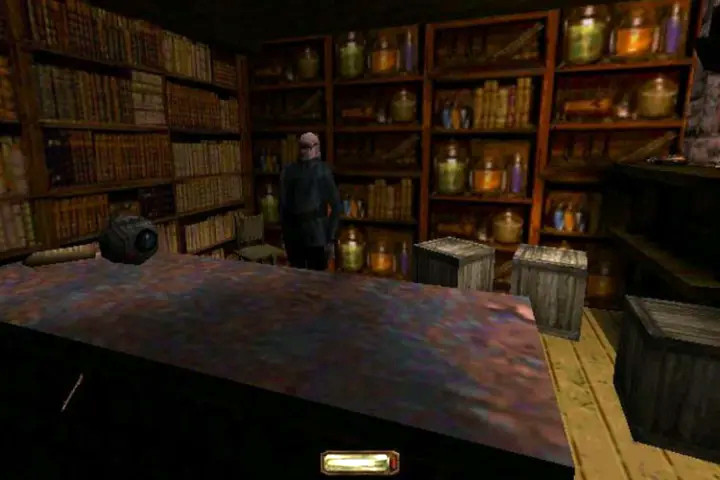
\includegraphics[width=\linewidth]{images/thief.jpg}
        \caption{Thief, 1998 utilise une architecture ECS}
    \end{subfigure}
    \hfill
    \begin{subfigure}{0.4\linewidth}
        \centering
        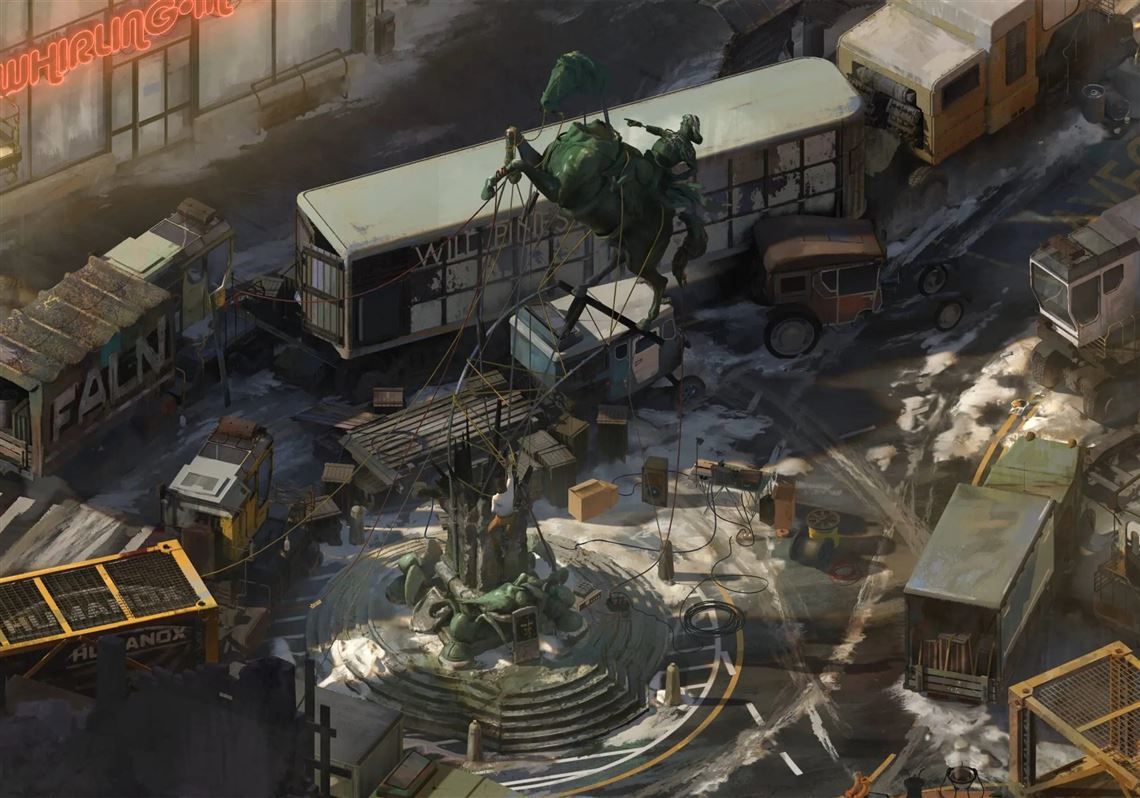
\includegraphics[width=\linewidth]{images/discoelysium-jpeg.jpeg}
        \caption{Disco Elysium, 2019, utilise une architecture Entity-Component sur le moteur Unity}
    \end{subfigure}
\end{figure}

Pour faire notre choix parmi toutes ces possibilités (et davantage encore!), nous avons dressé un cahier le cahier des charges de notre jeu : Tout d'abord, nous devions pouvoir afficher et mettre à jour \textbf{plusieurs centaines d'entités} sans chute majeure de performances. Nous avions besoin de pouvoir recevoir du serveur un \textbf{flux constant} de données et de le propager dans le jeu. Nos entités seraient peu complexes (non-nécessité d'une hiérarchie d'entités), et peu variées dans leur logique (préférence pour une approche \textit{data-driven}).





\subsubsection{Entity-component-system}
    L'architecture Entité-Composant-Système (souvent abrégé ECS) est une architecture permettant de décrire des entités en séparant totalement les données des traitements. Comme son nom l'indique, l'ECS est basé sur trois concepts clés :

\begin{itemize}
    \item \textbf{Les entités} (dans le jargon ECS) représentent exactement ce que l'on a appelé jusqu'ici "entité" : \textit{quelque chose} qui est dans le monde du jeu. Par elles mêmes, elles ne contiennent ni logique ni donnée, mais elle sont chacune associées à un ensemble de composants.
    \item \textbf{Les composants} sont des conteneurs de données typés. Leur type indique la fonction de leurs données. Par exemple, un composant 'Rendu' pourra contenir un maillage 3D et un composant 'Transformation', une matrice de $M_4(\mathbb R)$. Les composants ne contiennent aucune logique, mais c'est les systèmes qui vont exploiter leurs données.
    \item \textbf{Les systèmes} sont des fonctions qui agissent sur les entités de manière régulière ou ponctuelle. Chaque système n'agit que sur un sous-ensemble des entités qui possèdent les composants nécessaire à l'application du système. Par exemple, un système "Affichage3D" pourrait agir sur toutes les entités ayant au moins les composants "Rendu" et "Transformation".
\end{itemize}

    \begin{figure}[!h]
        \centering
        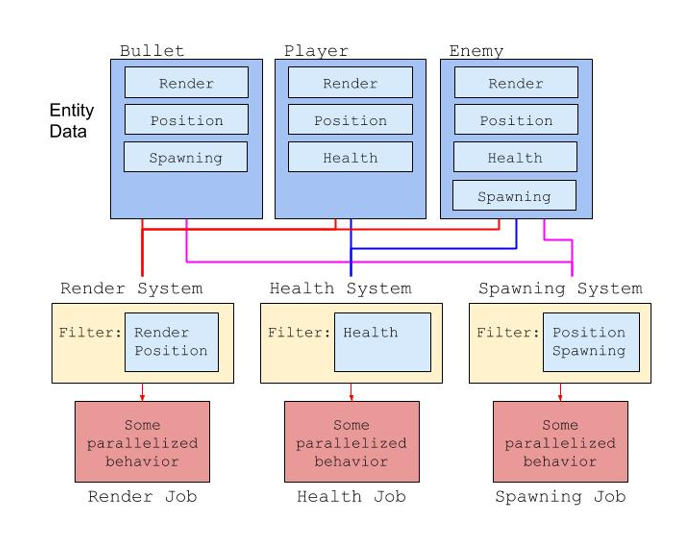
\includegraphics[width=0.5\linewidth]{images/ecsDiagram.PNG}
        \caption{Diagramme produit par Intel illustrant une architecture ECS}
        \label{fig:enter-label}
    \end{figure}

    Les avantages de l'ECS sont aussi nombreux que ses problèmes. La centralisation des traitements permet de gagner en performance lorsque le nombre d'entités est bien plus grand que le nombre de systèmes (donc que chaque système agit sur beaucoup d'entités en moyenne). En outre, la concentration des données dans les composants permet une approche \textit{data-driven}
        \footnote{"régie par les données". Paradigme de programmation où les données sont spécifiées en amont des traitements. Le langage de transformation XML \href{http://www.overleaf.com}{XSLT} en est un exemple.}
    D'un autre côté, pour des cas d'utilisation avec peu d'entités et beaucoup de variance dans la logique de traitement, l'ECS est peu souhaitable car il est moins intuitif à utiliser que la plupart des alternatives, et les gains de performance sont moindres voir négatifs.

    Nous utilisons une architecture ECS car ses forces coïncident avec notre cas d'utilisation : Traitement de beaucoup d'entités avec un nombre de traitement relativement restreint, et spécialisation d'un grand nombre d'entités par une approche orientée-données.


\subsubsection{Notre moteur}
    Pour rappel, nous avons choisi de développer notre propre moteur en \textit{typescript}, en utilisant la librairie de rendu 3D \textit{ThreeJS}.

    ThreeJS nous offre une interface haut niveau vers le WebGL. En d'autres termes, on lui délègue le rendu graphique. Cependant, le reste des concepts servant de base au jeu doivent être implémentés par nos soins. On décide de créer un moteur de jeu basique, spécialisé pour le jeu que l'on crée (en opposition à un moteur généraliste comme Godot ou Unreal Engine). Ce moteur est composé de plusieurs modules :
    
\begin{itemize}
    \item \textbf{ECS}
    \item \textbf{Components}
    \item \textbf{Systems}
    \item \textbf{Input}
    \item \textbf{User Interface}
    \item \textbf{Game}
\end{itemize} 

    Ces modules fonctionnent ensemble pour fournir une base solide à la création du jeu. Expliquons chacun d'eux en détails.
\paragraph{ECS}
    Notre implémentation de l'architecture ECS est basée sur \href{https://maxwellforbes.com/posts/typescript-ecs-implementation/}{\textit{cet article de 2021 écrit par Maxwell Forbes}}. Les entités sont simplement représentées par un entier. La classe \textit{ECS} lie ces identifiants à un ensemble d'objets héritant de \textit{Component}. La classe \textit{ECS} contient aussi l'ensemble des systèmes.
    
    Quand un système, une entité ou un composant est ajouté(e) ou enlevé(e) l'ECS, la liste des entités concernées par chaque système est mise à jour.
    Une fonction permet d'appliquer le traitement de chaque système aux entités concernées. Voici un exemple-jouet d'utilisation de notre système ECS pour faire rebondir des objets sur le sol.

    TODO EXEMPLE DE CODE


    Nous définissons une liste de composants et systèmes "\textit{Core}" : des éléments généraux et fondamentaux au jeu. Comme notre moteur est très lié à notre jeu, cette frontière n'est pas toujours claire, par exemple, le code de synchronisation avec le serveur et le code d’interaction joueur-monde sont tous deux définis dans le jeu. Ils seront explicités dans la partie suivante qui portera sur le jeu en lui même.
\paragraph{Components (\textit{Core})}
    TODO


\paragraph{Systems (\textit{Core})}
    TODO




\paragraph{Input}
    TODO
    


\paragraph{Game (Classe)}
    TODO